% Template for Cogsci submission with R Markdown

% Stuff changed from original Markdown PLOS Template
\documentclass[10pt, letterpaper]{article}

\usepackage{cogsci}
\usepackage{pslatex}
\usepackage{float}
\usepackage{caption}

% amsmath package, useful for mathematical formulas
\usepackage{amsmath}

% amssymb package, useful for mathematical symbols
\usepackage{amssymb}

% hyperref package, useful for hyperlinks
\usepackage{hyperref}

% graphicx package, useful for including eps and pdf graphics
% include graphics with the command \includegraphics
\usepackage{graphicx}

% Sweave(-like)
\usepackage{fancyvrb}
\DefineVerbatimEnvironment{Sinput}{Verbatim}{fontshape=sl}
\DefineVerbatimEnvironment{Soutput}{Verbatim}{}
\DefineVerbatimEnvironment{Scode}{Verbatim}{fontshape=sl}
\newenvironment{Schunk}{}{}
\DefineVerbatimEnvironment{Code}{Verbatim}{}
\DefineVerbatimEnvironment{CodeInput}{Verbatim}{fontshape=sl}
\DefineVerbatimEnvironment{CodeOutput}{Verbatim}{}
\newenvironment{CodeChunk}{}{}

% cite package, to clean up citations in the main text. Do not remove.
\usepackage{apacite}

% KM added 1/4/18 to allow control of blind submission


\usepackage{color}

% Use doublespacing - comment out for single spacing
%\usepackage{setspace}
%\doublespacing


% % Text layout
% \topmargin 0.0cm
% \oddsidemargin 0.5cm
% \evensidemargin 0.5cm
% \textwidth 16cm
% \textheight 21cm

\title{Children and adults integrate social and stastical information seeking
during language processing}

\usepackage{threeparttable}
\usepackage{booktabs}

\author{{\large \bf Kyle MacDonald (kemacdonald@ucla.edu)} \\ Department of Communication, UCLA  \AND {\large \bf Elizabeth Swanson (elizswan@stanford.edu)} \\ Department of Psychology, Stanford University  \AND {\large \bf Michael C. Frank (mcfrank@stanford.edu)} \\ Department of Psychology, Stanford University  }

\begin{document}

\maketitle

\begin{abstract}
How do children learn words from input that has many possible
word-object mappings? Statistical learning allows children to aggregate
consistent word-object co-occurrences to reduce uncertainty over time,
while social-pragmatic cues can constrain ambiguity within a labeling
event. Here, we present two eye-tracking studies that ask how learners
integrate statistical and social information during real-time language
processing. When processing familiar words, children and adults did not
delay their gaze shifts to seek a post-nominal social cue to reference
(eye gaze). When processing novel words, however, children and adults
fixated longer on a speaker who produced a gaze cue, which, in turn, led
to an increase in looking to a named object and less looking to the
other object in the scene. These results suggest that learners integrate
their knowledge of object labels when deciding how to allocate visual
attention to social partners, which in turn can shape the input to word
learning mechanisms.

\textbf{Keywords:}
eye movements; language processing; information-seeking; word learning;
gaze following
\end{abstract}

\hypertarget{introduction}{%
\section{Introduction}\label{introduction}}

People use language to talk about many things, with no guarantee that
they refer to objects in the co-occurring visual context. The
flexibility of language creates a challenge where learners often
encounter new words whose intended meanings are mostly unconstrained.
But children are quite capable word learners. How does word learning
unfold despite ambiguity in the input?

Research on lexical development has pursued several solutions. Lab-based
studies and computational models show that learners can overcome
referential uncertainty within a labeling event by tracking the elements
of a context that remain consistent across multiple exposures to a new
word (cross-situational learning) (Roy \& Pentland, 2002; Yu \& Smith,
2007). Social-pragmatic accounts highlight research showing that
children's social partners reduce the complexity of the learning task by
using gesture and eye gaze to coordinate language interactions with
children (Bloom, 2002; Estigarribia \& Clark, 2007). Moreover, even
16-month-olds can use cues from other people (e.g., the direction of
their gaze) to infer the meaning of a new word (Baldwin, 1993).

Both social and statistical information can reduce uncertainty about
reference during language processing. These processes, however, do not
operate in isolation, and a sophisticated learner might integrate
information from both sources to learn words. Computational models show
better learning by integrating social information with cross-situational
learning mechanisms (Frank, Goodman, \& Tenenbaum, 2009; Yu \& Ballard,
2007).

The statistical and social accounts of word learning reviewed above
reflect a somewhat passive construal of the learner. Children, however,
take actions to shape learning (e.g., choosing where to look or point).
Empirical work shows that ``active'' control can speed learning because
it allows people to integrate prior knowledge and uncertainty to seek
more useful information (Gureckis \& Markant, 2012). For example,
Kachergis, Yu, \& Shiffrin (2013) found that adults who selected objects
to be labeled learned more word-object associations compared to adults
who passively experienced labels.

Here, we pursue an active, integrative account and ask how children's
social information seeking changes as they experience multiple exposures
to a word-object link. Our second goal is to test whether children and
adults would show a similar pattern of adaptation to gather a social cue
to reference. It could be that children rely more on information from
social partners because they have to understand and learn language
despite having partial knowledge of word-object links and without a
fully-developed language model. Moreover, adults have stronger
statistical word learning skill, which could diminish the usefulness of
seeking a social cue to reference when they detect a consistent
association between a word and object.

\begin{CodeChunk}
\begin{figure*}[h]

{\centering 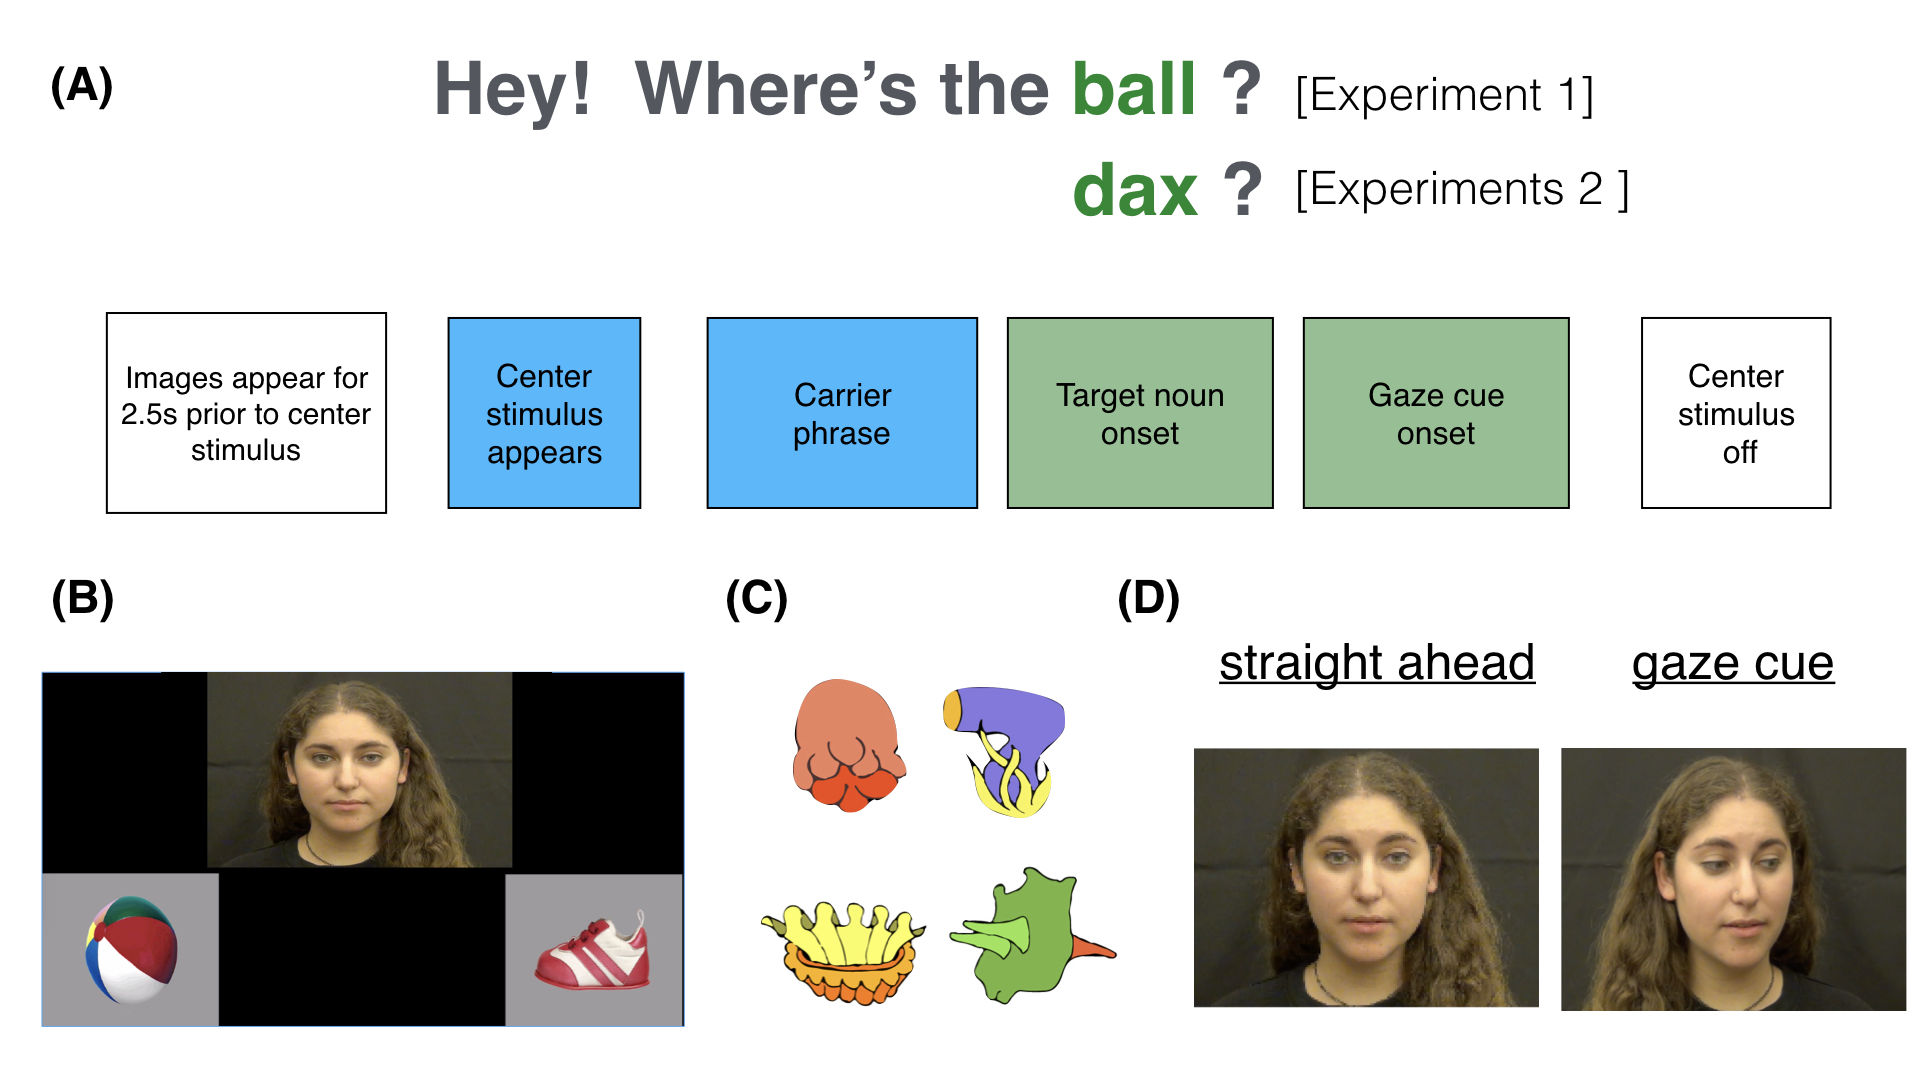
\includegraphics[width=0.65\linewidth]{/Users/kylemacdonald/Documents/Projects/SPEED-ACC-NOVEL/writing/figures/plots/gaze_stimuli} 

}

\caption[Stimuli for Experiments 1 and 2]{Stimuli for Experiments 1 and 2. Panel A shows the structure of the linguistic stimuli for a single trial. Panel B shows the layout of the fixation locations for all tasks: the center stimulus, the target, and the distracter. Panel C shows a sample of the images used as novel objects in Experiment 2. Panel D shows an example of the social gaze manipulation.}\label{fig:gaze-stimuli}
\end{figure*}
\end{CodeChunk}

In our experiments, we analyze fixations to a speaker's face who either
does or does not provide a valid cue to reference: eye gaze. We chose
this behavior as a case study of social information seeking because gaze
following is thought to be relevant for the ecological task of linking
language to the world. Moreover, recent work has found a reliable link
between sustained visual attention on objects and word learning (Smith
\& Yu, 2013). In Experiment 1, we explore social information seeking in
the context of processing concrete, familiar words, where we assume
prior exposure to statistical information about word-object links
outside the lab. Experiment 2 extends our approach to the case of novel
word learning, allowing us to control the number of exposure to a new
word and ask whether social information seeking becomes more useful in
contexts with more uncertainty.

We characterize eye movements as a series of information seeking
decisions that aim to minimize uncertainty (Hayhoe \& Ballard, 2005).
Using this account, children should integrate statistical and social
information by considering the utility of an eye movement for their
current goal. We hypothesized that when a communicative partner produces
a social cue to reference, they increase the value of looking to the
speaker for the task of disambiguating reference. Our key behavioral
prediction is that listeners will delay generating an eye movement away
from a speaker until they have gathered information about the direction
of their gaze. This delay will lead to an increase in fixations to the
named object, which, in turn, could change the time course of
statistical word learning.

\hypertarget{experiment-1}{%
\section{Experiment 1}\label{experiment-1}}

In Experiment 1, we measured the time course of children and adults'
decisions about visual fixation as they processed sentences with
familiar words (``Where's the ball?''). We manipulated whether the
speaker produced a post-nominal gaze cue to the named object. The visual
world consisted of three fixation targets (a center video of a person
speaking, a target picture, and a distracter picture; see Figure 1). The
primary question of interest is whether listeners would delay shifting
their gaze away from the speaker's face when she was likely to generate
a gaze cue. We predicted that fixating longer on the speaker would allow
listeners to gather more language-relevant visual information to
facilitate comprehension. In contrast, if listeners show parallel gaze
dynamics across the gaze and no-gaze conditions, this pattern suggests
that hearing the familiar word was the primary factor driving shifts in
visual attention.

\begin{CodeChunk}
\begin{figure*}[t]

{\centering 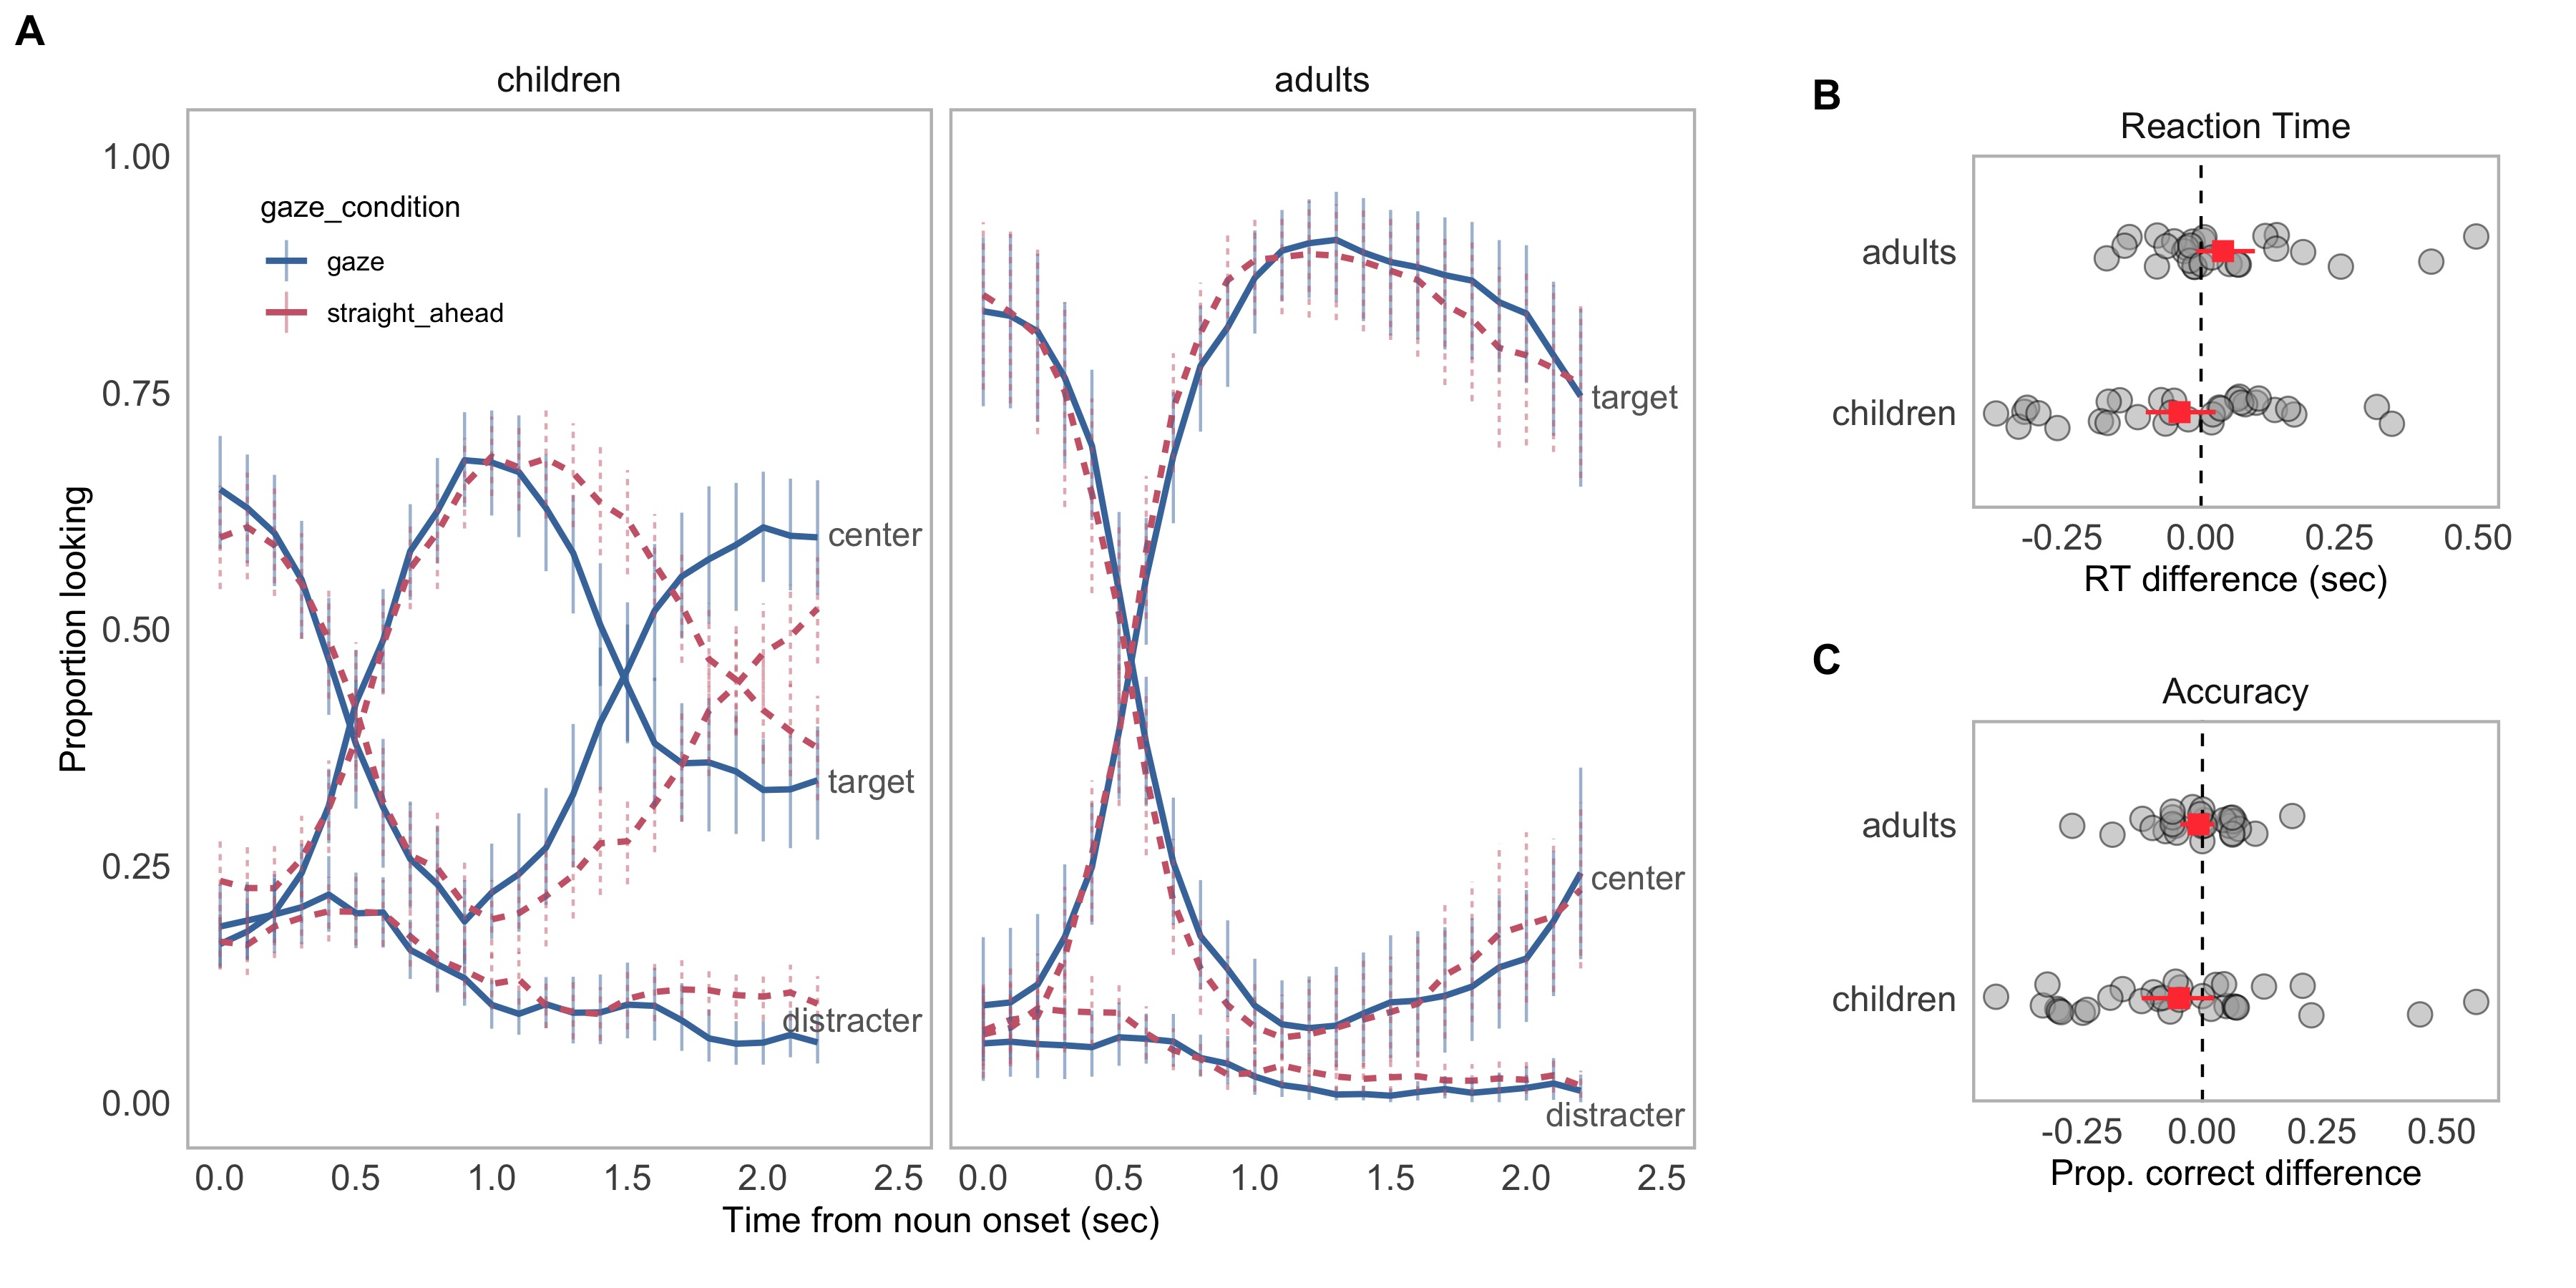
\includegraphics[width=0.85\linewidth]{/Users/kylemacdonald/Documents/Projects/SPEED-ACC-NOVEL/writing/figures/plots/speed_acc_fam_behav} 

}

\caption[Timecourse looking, first shift Reaction Time (RT), and Accuracy results for children and adults in Experiment 1]{Timecourse looking, first shift Reaction Time (RT), and Accuracy results for children and adults in Experiment 1. Panel A shows the overall looking to the center, target, and distracter stimulus for each gaze condition and age group. Panel B shows the distribution of pairwise contrasts between each participant's RT in the gaze and no-gaze conditions. The square point represents the group means. The vertical dashed line represents the null model of zero condition difference. Error bars represent the 95\% HDI. Panel C shows the same information but for first shift accuracy.}\label{fig:speed-acc-gaze-results}
\end{figure*}
\end{CodeChunk}

\hypertarget{analytic-approach}{%
\subsection{Analytic approach}\label{analytic-approach}}

To quantify evidence for our predictions, we present two analyses.
First, we analyze the time course of listeners' looking to each area of
interest (AOI). Proportion looking reflects the mean proportion of
trials on which participants fixated on the speaker, the target image,
or the distracter image at every 33-ms interval of the stimulus
sentence. We tested condition differences in the proportion looking to
the language source -- signer or speaker -- using a nonparametric
cluster-based permutation analysis, which accounts for the issue of
taking multiple comparisons across many time bins in the timecourse
(Maris \& Oostenveld, 2007). A higher proportion of looking to the
language source in the gaze condition would indicate listeners'
prioritization of seeking visual information from the speaker.

Next, we analyzed the RT and Accuracy of participants' initial gaze
shifts away from the speaker to objects in the scene. RT corresponds to
the latency of shifting gaze away from the central stimulus to either
object measured from the onset of the target noun. All reaction time
distributions were trimmed to between zero and two seconds, and RTs were
modeled in log space. Accuracy corresponds to whether participants'
first gaze shift landed on the target or the distracter object. If
listeners generate slower but more accurate gaze shifts, this provides
evidence that gathering more visual information from the speaker led to
more robust language processing in the gaze context.

We used the \texttt{brms} (Bürkner, 2017) package to fit Bayesian
mixed-effects regression models. The mixed-effects approach allowed us
to model the nested structure of our data -- multiple trials for each
participant and item, and the within-participants manipulation. We used
Bayesian estimation to quantify uncertainty in our point estimates,
which we communicate using a 95\% Highest Density Interval (HDI),
providing a range of credible values given the data and model.

\hypertarget{methods}{%
\subsection{Methods}\label{methods}}

\hypertarget{participants}{%
\subsubsection{Participants}\label{participants}}

\begin{table}[tbp]
\begin{center}
\begin{threeparttable}
\caption{\label{tab:make-ss-table}Age distributions of children in Experiments 1 and 2. All ages are reported in months.}
\begin{tabular}{lllll}
\toprule
Experiment & \multicolumn{1}{c}{n} & \multicolumn{1}{c}{Mean} & \multicolumn{1}{c}{Min} & \multicolumn{1}{c}{Max}\\
\midrule
Exp. 1 (familiar words) & 38 & 55.50 & 35.60 & 71.04\\
Exp. 2 (novel words) & 54 & 52.60 & 36.26 & 70.94\\
\bottomrule
\end{tabular}
\end{threeparttable}
\end{center}
\end{table}

Participants were native, monolingual English-learning children (\(n=\)
38; 19 F) and adults (\(n=\) 33; 23 F). All participants had no reported
history of developmental or language delay and normal vision. 12
participants (9 children, 3 adults) were run but not included in the
analysis because either the eye tracker failed to calibrate (8 children,
2 adults) or the participant did not complete the task (1 children, 1
adults).

\hypertarget{materials}{%
\subsubsection{Materials}\label{materials}}

\emph{Linguistic stimuli.} The video/audio stimuli were recorded in a
sound-proof room and featured two female speakers who used natural
child-directed speech and said one of two phrases: ``Hey! Can you find
the (target word)'' or "Look! Where's the (target word). The target
words were: ball, bunny, boat, bottle, cookie, juice, chicken, and shoe.
The target words varied in length (shortest = 411.68 ms, longest =
779.62 ms) with an average length of 586.71 ms.

\emph{Gaze manipulation}. To create the stimuli in the gaze condition,
the speaker waited until she finished producing the target sentence and
then turned her head to gaze at the bottom corner of the camera frame.
After looking at the named object, she then returned her gaze to the
center of the frame. We chose to allow the length of the gaze cue to
vary to keep the stimuli naturalistic. The average length of gaze was
2.12 seconds with a range from 1.78 to 3.07 seconds.

\emph{Visual stimuli.} The image set consisted of colorful digitized
pictures of objects presented in fixed pairs with no phonological
overlap between the target and the distracter image (cookie-bottle,
boat-juice, bunny-chicken, shoe-ball). The side of the target picture
was counterbalanced across trials.

\hypertarget{procedure}{%
\subsubsection{Procedure}\label{procedure}}

Participants viewed the task on a screen while their gaze was tracked
using an SMI RED corneal-reflection eye-tracker mounted on an LCD
monitor, sampling at 30 Hz. The eye-tracker was first calibrated for
each participant using a 6-point calibration. On each trial,
participants saw two images of familiar objects on the screen for two
seconds before the center stimulus appeared. Next, they processed the
target sentence followed by two seconds without language to allow for a
response. Both children and adults saw 32 trials (16 gaze trials; 16
no-gaze trials) with several filler trials interspersed to maintain
interest. The gaze manipulation was presented in a blocked design with
the order of block counterbalanced across participants.

\hypertarget{results-and-discussion}{%
\subsection{Results and Discussion}\label{results-and-discussion}}

\hypertarget{timecourse-looking}{%
\subsubsection{Timecourse looking}\label{timecourse-looking}}

We first analyzed how the presence of gaze influenced listeners'
distribution of attention across the three fixation locations. At
target-noun onset, listeners tended to look more at the speaker than the
objects. As the target noun unfolded, the mean proportion looking to the
center decreased as participants shifted their gaze to the images. After
looking to the named referent, listeners tended to shift their gaze back
to the speaker's face.

We did not see evidence that the presence of a post-nominal gaze cue
changed how children or adults allocated attention early in the target
word. Children in the gaze condition, however, tended to shift their
focus back to the speaker earlier after shifting gaze to the named
object and spent more time fixating on the speaker's face throughout the
rest of the trial (\(p < .001\)).

\hypertarget{first-shift-rt-and-accuracy}{%
\subsubsection{First shift RT and
Accuracy}\label{first-shift-rt-and-accuracy}}

Both children and adults generated similar RTs in the gaze (children
\(M_{rt}\) = 563.159 ms, adults \(M_{rt}\) = 652.405 ms) and no-gaze
(children \(M_{rt}\) = 575.762 ms, adults \(M_{rt}\) = 608.314 ms)
conditions, with the null value of zero condition differences falling
within the 95\% credible interval (\(\beta\) = -0.36, {[}-0.89,
0.06{]}). Next, we fit the same model to estimate first shift accuracy.
Adults generated more accurate gaze shifts (\(M\) = 0.9) compared to
children (\(M\) = 0.64) with the null value falling outside the 95\% HDI
(\(\beta_{age}\) = -1.76, {[}-2.19, -1.34{]}). Similar to the RT
analysis, we did not find evidence of a difference in performance across
the gaze conditions (\(\beta\) = 0.10, {[}-0.18, 0.41{]}).

The time course and first shift analyses suggest that hearing a familiar
noun was sufficient for both adults and children to shift visual
attention away from the speaker to seek a named referent. Neither age
group showed evidence of delaying eye movements to gather a social cue
to reference. Children, however, did allocate more attention to the
speaker after processing the familiar noun. While we did not predict
these results, this behavior seems reasonable if eye movements during
familiar language processing are highly-practiced visual routines such
that seeking a post-nominal gaze cue becomes less-relevant for
disambiguating reference.

The results of Experiment 1 suggest that listeners do not always seek
social information when it is available; instead, they might take their
uncertainty into account and use social information when ambiguity is
higher. This interpretation raises an interesting question: Would
listeners adapt to gather social information when they do not already
know the meaning of a word? That is, when surrounded by unfamiliar
objects, the value of fixating on a social partner may increase since
this action could provide access to useful disambiguating information
such as eye gaze-- an idea emphasized by social-pragmatic theories of
language acquisition (Bloom, 2002).

\hypertarget{experiment-2}{%
\section{Experiment 2}\label{experiment-2}}

Experiment 2 explores whether learners will adapt the timing of gaze
shifts to seek information from social partners when encountering a
novel word. We ask three research questions: (1) do listeners adapt
their gaze to seek social information in the context of processing novel
words? (2) Does social information seeking change as a function of
gaining more exposures to a word-object association? And (3) does
following a gaze cue enhance learning of a novel word-object link? To
answer these questions, we compared the timing and accuracy of eye
movements during a real-time cross-situational word learning task where
participants processed sentences containing a novel word (``Where's the
dax?'').

We predicted that the presence of gaze would increase the value of
looking to a speaker, leading to a higher proportion of fixations to the
social target and slower first shift reaction times to the objects. We
operationalize this prediction as a main effect of gaze condition on
proportion looking to the speaker and first shift RT. We also predict a
trial number by gaze condition interaction such that the decrease in RT
will be greater on exposure trials in the gaze condition, reflecting a
reductino in the need to seek social information after learning the
word-object mappings. Finally, we predicted that the presence of gaze
would lead to faster learning of the novel word-object links, which we
operationalize as more accurate first shifts, faster RTs, and a higher
proportion looking to the target object on test trials in the gaze
condition.

\begin{CodeChunk}
\begin{figure*}[t]

{\centering 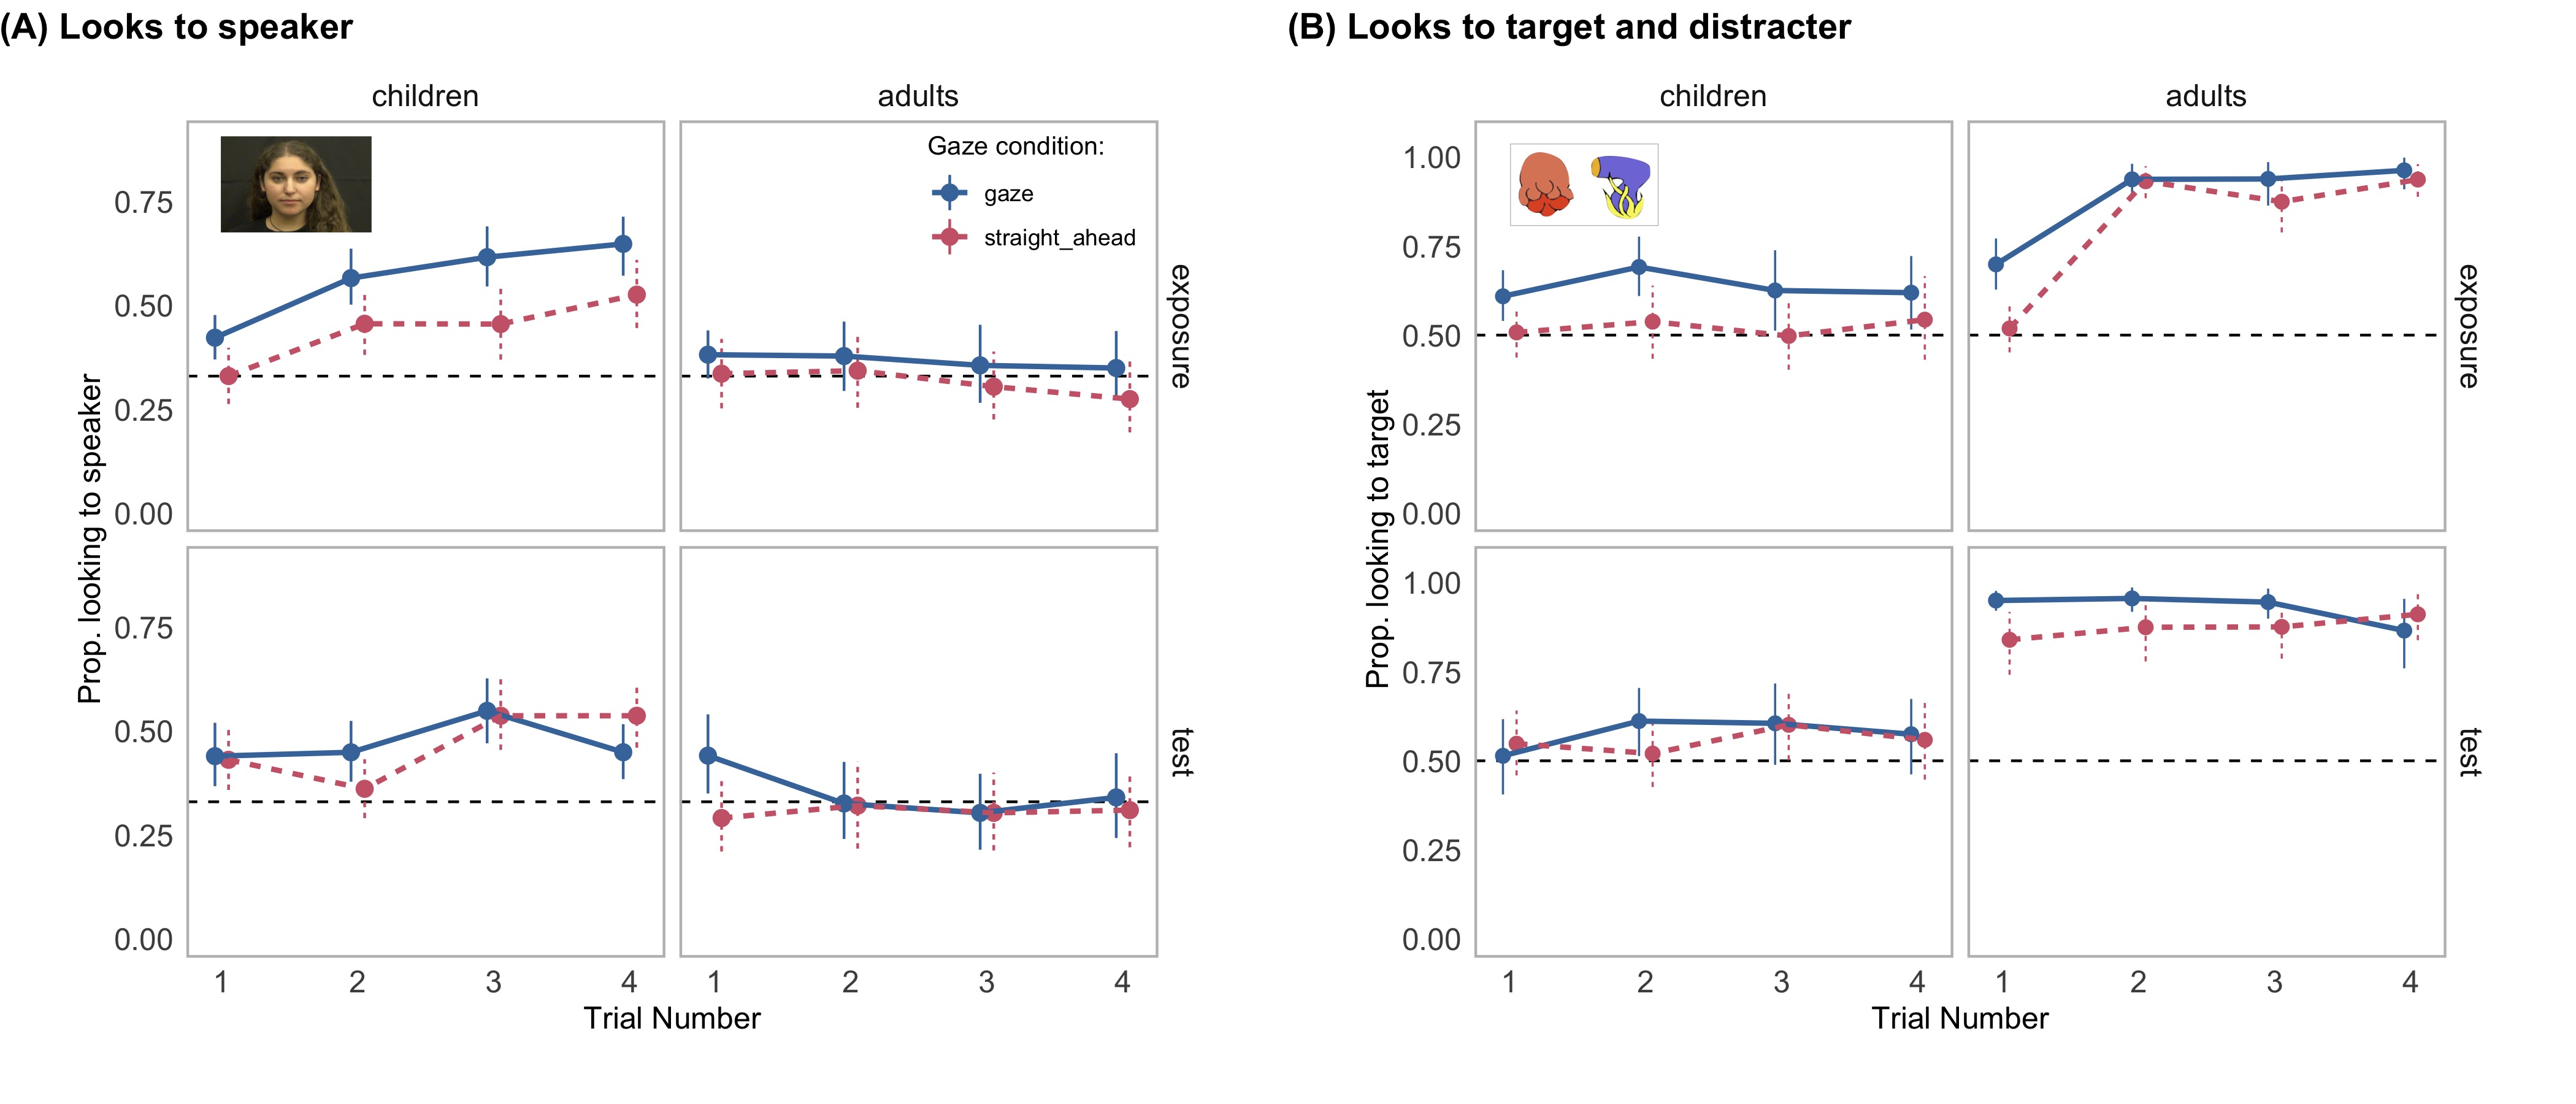
\includegraphics[width=0.95\linewidth]{/Users/kylemacdonald/Documents/Projects/SPEED-ACC-NOVEL/writing/figures/plots/speed_acc_novel_proplook} 

}

\caption[Panel A shows participants’ tendency to look at the speaker on exposure and test trials as a function of the trial number within a learning block]{Panel A shows participants’ tendency to look at the speaker on exposure and test trials as a function of the trial number within a learning block. The horizontal, dashed line represents the tendency to distribute attention equally across the three AOIs. Color indicates gaze condition and error bars represent 95\% credible intervals. Panel B shows the same information but for target and distracter looking across the learning block.}\label{fig:san-prop-looking-plot}
\end{figure*}
\end{CodeChunk}

\hypertarget{methods-1}{%
\subsection{Methods}\label{methods-1}}

\hypertarget{participants-1}{%
\subsubsection{Participants}\label{participants-1}}

Participants were native, monolingual English-learning children (\(n=\)
54; 30 F) and adults (\(n=\) 30; 20 F). All participants had no reported
history of developmental or language delay and normal vision. 6 adults
were run but not included in the analysis because they were not native
speakers of English. 7 children participants were run but not included
in the analysis because the participant did not complete more than half
of the trials in the task.

\hypertarget{materials-1}{%
\subsubsection{Materials}\label{materials-1}}

\emph{Linguistic stimuli.} The video/audio stimuli were recorded in a
sound-proof room and featured two female speakers who used natural
child-directed speech and said one of two phrases: ``Hey! Can you find
the (novel word)'' or "Look! Where's the (novel word). The target words
were four pseudo-words: bosa, modi, toma, and pifo. The novel words
varied in length (shortest = 472.00 ms, longest = 736.00 ms) with an
average length of 606.31 ms.

\emph{Gaze manipulation}. The gaze manipulation was identical to
Experiment 1. The average length of gaze was 2.06 seconds with a range
from 1.74 to 2.67 seconds.

\emph{Visual stimuli.} The image set consisted of 28 colorful digitized
pictures of objects that were selected such that they would be
interesting to and that children would be unlikely to have already a
label associated with the objects. The side of the target picture was
counterbalanced across trials.

\hypertarget{procedure-1}{%
\subsubsection{Procedure}\label{procedure-1}}

The procedure was identical to Experiment 1. Participants watched a
series of ambiguous word learning events organized into pairs of one
exposure and one test trial. On each trial, participants saw a set of
two unfamiliar objects and heard one novel word. Each word occurred in a
block of four exposure-test pairs for a total of eight trials for each
novel word. On each trial within a learning block, one of the objects in
the set had consistently appeared on the previous trials (target
object), while the other object was a randomly generated novel object
that had not been shown in the experiment (distracter object).

\hypertarget{results-and-discussion-1}{%
\subsection{Results and Discussion}\label{results-and-discussion-1}}

\hypertarget{proportion-looking}{%
\subsubsection{Proportion looking}\label{proportion-looking}}

\emph{Learning effects.} Both children (\(M_{gaze}\) = 0.57,
\(M_{no-gaze}\) = 0.55) and adults (\(M_{gaze}\) = 0.91, \(M_{no-gaze}\)
= 0.89) showed evidence of learning the novel word-object links, with
the null value of 0.5 falling below the lower bound of the lowest
credible interval for children's target looking in the No-gaze context
(95\% HDI {[}0.51, 0.60{]}). Our primary question of interest was how
exposure to multiple co-occurrences of word-object pairs would change
learners' distribution of attention between the speaker and objects.
Both children and adults were more likely to fixate on the speaker when
she provided a gaze cue (\(\beta_{gaze}\) = 0.09 {[}0.16, 0.01{]}).
Moreover, there was a developmental difference such that children, but
not adults, were more likely to increase their fixations to the speaker
over the course of the learning block (Fig 4A, \(\beta_{age*tr.num}\) =
-0.07, {[}-0.11, -0.04{]}).

Overall, looking to the target increased as learners were exposed to
more word-object pairings (\(\beta_{tr.num}\) = 0.16, {[}0.09, 0.24{]})
and was higher when the novel word was accompanied by a gaze cue
(\(\beta_{gaze}\) = 0.14, {[}0.21, 0.06{]}). Visual inspection of the
top row of Fig \ref{fig:san-prop-looking-plot}B shows that on the first
exposure trial, both adults and children used the gaze cue to
disambiguate reference, fixating more on the target in the gaze
condition. For children, higher target looking on exposure trials with
gaze remained relatively constant across the learning block. In
contrast, adults target looking reached ceiling for both the gaze and
no-gaze conditions by trial number two, indicating that they had
successfully used co-occurrence information to learn the words. For
adults, we found an interaction between gaze condition and trial number
such that looking to the target increased more quickly in the No-gaze
condition (\(\beta_{gaze*tr.num}\) = 0.02, {[}0.00, 0.04{]}), which
reflects (1) the higher intercept of target looking in the presence of
gaze and (2) rapid learning of the word-object association via
cross-situational information (bottom row of Fig 4B). Finally, visual
inspection of test trials in Fig 4B suggests that adults tended to look
more the target when learning from a gaze cue, only reaching similar
levels of accuracy in the no-gaze condition at the end of the learning
block. There was not strong evidence that the gaze manipulation
influenced children's looking behavior on test trials.

\emph{Relationship between looking on exposure and test.} For both
children and adults, more time attending to the target object on
exposure trials led to a higher proportion of looking to the target on
test trials, especially for adults (\(\beta_{exposure*age}\) = 0.16,
{[}0.05, 0.28{]}) and as the number of word-object exposures increased
over the course a learning block (\(\beta_{exposure*tr.num}\) = 0.07,
{[}0.02, 0.12{]}). There was evidence that participants in the No-gaze
condition showed less learning over the course of the word block
(\(\beta_{gaze*tr.num}\) = -0.02, {[}-0.04, 0.00{]}). This result
provides evidence that the presence of social information did more than
change attention on exposure trials but instead modulated the
relationship between attention during learning and later memory for
word-object links.

\hypertarget{first-shift-rt-and-accuracy-1}{%
\subsubsection{First shift RT and
Accuracy}\label{first-shift-rt-and-accuracy-1}}

We next asked how the presence of gaze influenced learners' decision to
stop gathering visual information from the speaker and start fixating on
the novel objects. Both children (Gaze \(M_{rt}\) = 1,136.77 ms, No-gaze
\(M_{rt}\) = 878.37 ms) and adults (Gaze \(M_{rt}\) = 878.65 ms, No-gaze
\(M_{rt}\) = 726.99 ms) fixated longer on the speaker when she provided
a gaze cue (\(\beta_{gaze}\) = -0.20, {[}-0.38, -0.01{]}). With no
evidence of an interaction between gaze condition and age group
(\(\beta_{age*gaze}\) = 0.27, {[}0.11, 0.44{]}). Moreover, both children
(Gaze \(M_{acc}\) = 0.64, No-gaze \(M_{acc}\) = 0.49) and adults (Gaze
\(M_{acc}\) = 0.89, No-gaze \(M_{acc}\) = 0.81) generated more accurate
first shifts in the gaze condition, indicating they were following the
gaze cue on exposure trials (\(\beta_{gaze}\) = -0.57, {[}-1.13,
0.00{]}).

Finally, we asked whether the presence of gaze affected learning by
predicting first shift accuracy on test trials. We found that adults
were more accurate than children (\(\beta_{age}\) = 2.24, {[}1.50,
3.03{]}), that first shifts became more accurate as learners experienced
repeated exposures to word-object pairings (\(\beta_{tr.num}\) = 0.21,
{[}-0.02, 0.44{]}). We did not see evidence for two of our predictions:
(1) that children and adults would generate more accurate first shifts
when learning from social gaze (\(\beta_{gaze}\) = -0.50, {[}-1.14,
0.14{]}) and (2) that learning from gaze would modulate the relationship
between accuracy over the course of learning (\(\beta_{gaze*tr.num}\) =
-0.30, {[}-0.74, 0.12{]}), with the null value falling within each
credible interval.

Returning to our three behavioral predictions, we found evidence that
both children and adults spent more time fixating on a speaker when she
provided a useful social cue to reference. Moreover, adults decreased
the amount of time fixating on the speaker as they gained more exposures
to the word-object pairings, but children showed the opposite pattern,
increasing their fixations to the speaker later in the task. This
developmental difference suggests that looking to a social partner may
have been more useful for children who were still trying to disambiguate
the novel words; whereas adults showed evidence of successful
disambiguation after the second exposure trial and could focus attention
on the objects instead. Finally, we found mixed evidence that the
presence of gaze modulated the relationship between visual attention
during labeling and learning of the novel word-object mappings. Both
children and adults generated a higher proportion of shifts landing on
the target when there was post-nominal gaze cue available. But only
adults spent more time fixating on the target object and generated more
accurate first shifts for words learned with a gaze cue.

\hypertarget{general-discussion}{%
\section{General Discussion}\label{general-discussion}}

Does social information seeking change as children gain more statistical
information about the link between a word and object? Here, we pursued
the idea that learners flexibly adapt their eye movements to gather
social gaze when it was useful. We found that children and adults did
not delay their gaze shifts to seek a post-nominal gaze cue while
processing familiar words. When processing novel words, however, both
children and adults fixated more on a speaker to seek a post-nominal
gaze cue. This delay resulted in more attention allocated to the named
object and less looking to the distracter object, an effect that
increased throughout the task for children. Moreover, adults, but not
children, showed evidence of stronger learning in the presence of social
gaze while both age groups were capable of learning the word-object
pairings from cross-situational statistics alone.

How should we characterize the effects of gaze on information seeking
and word learning in our task? Children selectively gathered social
information when they were uncertain about the meaning of a new word,
focusing attention on a single object. This pattern of behavior
generalized to trials without a gaze cue, showing how the effect of gaze
could accumulate over time. Finally, seeking social gaze increased the
rate of word learning for adults. This finding dovetails with other work
showing that the presence of social information changes information
processing (Wu, Gopnik, Richardson, \& Kirkham, 2011; Yoon, Johnson, \&
Csibra, 2008).

We did not find strong evidence that the effects of gaze generalized to
contexts without gaze for children in Experiment 2. Moreover, children
did not show strong learning of the novel word-object links overall.
Prior work has shown that 3-5 year-olds learn words better from an
extended, as opposed to brief, social cue to reference (Yurovsky, Wade,
\& Frank, 2013). Future work could increase the length of the gaze cue,
which was relatively short in these studies (\textasciitilde{}2 sec) or
could include a wider set of cues to reference such as pointing or
holding objects.

This work integrates social-pragmatic and statistical accounts of
language acquisition. We found that listeners' decisions to seek social
information varied depending on their uncertainty over word-object
mappings. In the context of processing novel, but not familiar words,
listeners adapted their gaze to seek a post-nominal social cue to
reference. This change led to increased visual attention on a single
object and less attention distributed across potential spurious
word-object links. Moreover, following gaze modulated the relationship
between attention during labeling and learning of word meaning. This
approach sheds light on how children might integrate social and
statistical information when deciding where to look, which, in turn,
shapes the information that comes into contact with statistical learning
processes.

\vspace{1em}

\fbox{\parbox[b][][c]{7.3cm}{\centering Data/code available at \url{https://bit.ly/2FgIbsW} \\ E1 preregistration at \url{https://osf.io/2q4gw/}\\ E2 preregistration at \url{https://osf.io/nfz85/}}}
\vspace{1em}

\hypertarget{acknowledgements}{%
\section{Acknowledgements}\label{acknowledgements}}

We are grateful to the people who participated in this research. Thanks
to Kayla Constandse, Tami Alade, and Hannah Slater for help with data
collection. This work was supported by an NSF GRFP to KM and a Jacobs
Foundation Fellowship to MCF.

\hypertarget{references}{%
\section{References}\label{references}}

\setlength{\parindent}{-0.1in} 
\setlength{\leftskip}{0.125in}

\noindent

\hypertarget{refs}{}
\leavevmode\hypertarget{ref-baldwin1993infants}{}%
Baldwin, D. A. (1993). Infants' ability to consult the speaker for clues
to word reference. \emph{Journal of Child Language}, \emph{20}(02),
395--418.

\leavevmode\hypertarget{ref-bloom2002children}{}%
Bloom, P. (2002). \emph{How children learn the meaning of words}. The
MIT Press.

\leavevmode\hypertarget{ref-burkner2017brms}{}%
Bürkner, P.-C. (2017). Brms: An r package for bayesian multilevel models
using stan. \emph{Journal of Statistical Software}, \emph{80}(1), 1--28.

\leavevmode\hypertarget{ref-estigarribia2007getting}{}%
Estigarribia, B., \& Clark, E. V. (2007). Getting and maintaining
attention in talk to young children. \emph{Journal of Child Language},
\emph{34}(4), 799--814.

\leavevmode\hypertarget{ref-frank2009using}{}%
Frank, M. C., Goodman, N. D., \& Tenenbaum, J. B. (2009). Using
speakers' referential intentions to model early cross-situational word
learning. \emph{Psychological Science}, \emph{20}(5), 578--585.

\leavevmode\hypertarget{ref-gureckis2012self}{}%
Gureckis, T. M., \& Markant, D. B. (2012). Self-directed learning a
cognitive and computational perspective. \emph{Perspectives on
Psychological Science}, \emph{7}(5), 464--481.

\leavevmode\hypertarget{ref-hayhoe2005eye}{}%
Hayhoe, M., \& Ballard, D. (2005). Eye movements in natural behavior.
\emph{Trends in Cognitive Sciences}, \emph{9}(4), 188--194.

\leavevmode\hypertarget{ref-kachergis2013actively}{}%
Kachergis, G., Yu, C., \& Shiffrin, R. M. (2013). Actively learning
object names across ambiguous situations. \emph{Topics in Cognitive
Science}, \emph{5}(1), 200--213.

\leavevmode\hypertarget{ref-maris2007nonparametric}{}%
Maris, E., \& Oostenveld, R. (2007). Nonparametric statistical testing
of eeg-and meg-data. \emph{Journal of Neuroscience Methods},
\emph{164}(1), 177--190.

\leavevmode\hypertarget{ref-roy2002learning}{}%
Roy, D. K., \& Pentland, A. P. (2002). Learning words from sights and
sounds: A computational model. \emph{Cognitive Science}, \emph{26}(1),
113--146.

\leavevmode\hypertarget{ref-smith2013visual}{}%
Smith, L. B., \& Yu, C. (2013). Visual attention is not enough:
Individual differences in statistical word-referent learning in infants.
\emph{Language Learning and Development}, \emph{9}(1), 25--49.

\leavevmode\hypertarget{ref-wu2011infants}{}%
Wu, R., Gopnik, A., Richardson, D. C., \& Kirkham, N. Z. (2011). Infants
learn about objects from statistics and people. \emph{Developmental
Psychology}, \emph{47}(5), 1220.

\leavevmode\hypertarget{ref-yoon2008communication}{}%
Yoon, J. M., Johnson, M. H., \& Csibra, G. (2008). Communication-induced
memory biases in preverbal infants. \emph{Proceedings of the National
Academy of Sciences}, \emph{105}(36), 13690--13695.

\leavevmode\hypertarget{ref-yu2007unified}{}%
Yu, C., \& Ballard, D. H. (2007). A unified model of early word
learning: Integrating statistical and social cues.
\emph{Neurocomputing}, \emph{70}(13), 2149--2165.

\leavevmode\hypertarget{ref-yu2007rapid}{}%
Yu, C., \& Smith, L. B. (2007). Rapid word learning under uncertainty
via cross-situational statistics. \emph{Psychological Science},
\emph{18}(5), 414--420.

\leavevmode\hypertarget{ref-yurovsky2013online}{}%
Yurovsky, D., Wade, A., \& Frank, M. (2013). Online processing of speech
and social information in early word learning. In \emph{Proceedings of
the annual meeting of the cognitive science society} (Vol. 35).

\bibliographystyle{apacite}


\end{document}
